\documentclass[twoside,a4paper,titlepage,openright,12pt]{article}
% \usepackage[left=1.5in, right=1in, top=1in, bottom=1in, headheight=13.6pt]{geometry}
% \usepackage[a4paper,width=150mm,top=25mm,bottom=25mm,bindingoffset=6mm]{geometry}

% \usepackage[margin=1in]{geometry}
% \documentclass[a4paper,twoside]{book}
% \documentclass[a4paper,titlepage,openright,12pt]{MSThesis}
\usepackage{graphicx}    
\usepackage{epsfig}   
%\usepackage[font=footnotesize]{subfig}
% \usepackage{subfig}
\usepackage{caption}
% \usepackage{subcaption}
\usepackage{booktabs}
\usepackage{float}
\usepackage{fancyhdr}                              
\usepackage{makeidx}
\usepackage[nottoc,notlot,notlof]{tocbibind}     
\usepackage{supertabular}
\usepackage{array}              
\usepackage{setspace} 
\usepackage{enumerate}
\usepackage{rotating}
\usepackage{moreverb}
\usepackage{tikz}
\usepackage{multirow}
\usepackage{amsmath}
\usepackage{amsthm}
\usepackage{amssymb}
\usepackage{captcont}
\usepackage{verbatim}
\usepackage{titlesec}
\usepackage{url}
\usepackage{hyperref}
\usepackage{listings}
\usepackage[inline]{enumitem}
%\usepackage[colorlinks=false]{hyperref}
\usepackage{lipsum}
\usepackage{lscape}
\usepackage{color}
\usepackage{xr}
\usepackage{float}
\usepackage{longtable}
\usepackage{wrapfig}
\usepackage{cleveref}
\usepackage[acronym,nomain]{glossaries}
%\usepackage{natbib}
\RequirePackage[numbers,square]{natbib} 
% \bibliographystyle{iitd}
\usepackage{amsmath} 
% \usepackage{indentfirst}
%\usepackage{geometry}
% \usepackage[algoruled]{algorithm2e}
% \usepackage[figure,algoruled]{algorithm2e}
% \usepackage[figure,boxruled]{algorithm2e}
%\setlength{\parindent}{1.0em}
%%%%%%%%%%%%%%%%%%%%%%%%%%%%%%%%%%%%%%%%%%%%%%%%%%%%%%%%%%%%%%%%

%%%%%%%%%%%%%%%%%%%%%%%%%%%%%%%%%%%%%%%%%%%%%%%%%%

\setlength{\parskip}{1ex plus 0.5ex minus 0.2ex}
\setlength{\textheight}{8.5in}
\pagestyle{fancy}
% with this we ensure that the chapter and section
% headings are in lowercase.
\renewcommand{\bibname}{References}
% \renewcommand{\chaptermark}[1]{\markboth{#1}{}}
\renewcommand{\sectionmark}[1]{\markright{\thesection\ #1}}
\fancyhf{} % delete current setting for header and footer
%\fancyhead[LE,RO]{\bfseries\thepage}
%\fancyhead[LO]{\bfseries\rightmark}
%\fancyhead[RE]{\bfseries\leftmark}
\rhead{\fancyplain{}{\thepage}} % predefined ()
\lhead{\fancyplain{}{\rightmark}} % 1. sectionname, 1.1 subsection name etc

%\rfoot{\bfseries\thepage}
%\rfoot{\fancyplain{}{\thepage}}
% \cfoot{\em $\copyright$ 2022, Indian Institute of Technology Delhi}
\renewcommand{\headrulewidth}{0.5pt}
\renewcommand{\footrulewidth}{0.5pt}
\addtolength{\headheight}{2.5pt} % make space for the rule

\fancypagestyle{plain}{%
\fancyhead{} % get rid of headers on plain pages
\fancyfoot{}
%\rfoot{\bfseries\thepage}
% \cfoot{\em $\copyright$ 2019, Indian Institute of Technology Delhi}
\renewcommand{\headrulewidth}{0pt} % and the line
}

%% The smart version of cleardouble page.
\let\origdoublepage\cleardoublepage
\newcommand{\clearemptydoublepage}{%
  \clearpage
  {\pagestyle{empty}\origdoublepage}%
}
\usepackage{xspace}
\newcommand{\Guide}{Sorav Bansal}
\newcommand{\Auth}{Indrajit Banerjee}
\newcommand{\Entry}{(2020CSY7569)}
% \newcommand{\ThesisTitle}{MACHINE LEARNING BASED METHOD FOR STROKE DETECTION AND STROKE TYPE IDENTIFICATION IN RESOURCE LIMITED ENVIRONMENT}

\newcommand{\ThesisTitle}{COUNTEREXAMPLE GUIDED EQUIVALENCE CHECKING BETWEEN PROGRAM SPECIFICATION USING SAFE ALGEBRAIC DATA TYPES AND ITS C IMPLEMENTATIONS}

\let\cleardoublepage\clearemptydoublepage


\date{}

\addtolength{\oddsidemargin}{30pt}
\addtolength{\evensidemargin}{-30pt}

\titlespacing*{\chapter}{0pt}{-50pt}{20pt}
\titleformat{\chapter}[display]{\normalfont\huge\bfseries}{\chaptertitlename\ \thechapter}{11pt}{\Huge}
\DeclareGraphicsExtensions{.pdf,.png,.jpg,.ps}
\restylefloat{figure}
\graphicspath{{./figures/}}

\usepackage{stackengine}
\usepackage{backnaur}
\usepackage{xcolor}
\usepackage{mathtools}
\usepackage{accents}

\newcommand{\xmark}{\ding{55}}%
\newcommand{\rulesep}{\unskip\ \vrule\ }

\setlength{\textfloatsep}{6.0pt plus 1.0pt minus 1.0pt}
\setlength{\intextsep}{3.0pt plus 0.5pt minus 0.5pt}

\makeatletter
\newcommand{\oset}[3][0ex]{%
  \mathrel{\mathop{#3}\limits^{
    \vbox to#1{\kern-2\ex@
    \hbox{$\scriptstyle#2$}\vss}}}}
\makeatother

\newcommand{\toolName}{S2C}%
\newcommand{\ite}[3]{\ensuremath{#1?#2:#3}}%
\newcommand{\sumDtor}{\underline{\tt if}-\underline{\tt then}-\underline{\tt else}}%
\newcommand{\sumIs}[2]{\ensuremath{#1\ \mathrm{is}\ \cons{#2}}}%
\newcommand{\fieldPath}[2][\ensuremath{.}]{%
  \def\nextitem{\def\nextitem{#1}}% Separator
  \renewcommand*{\do}[1]{\nextitem{\field{##1}}}% How to process each item
  \docsvlist{#2}% Process list
}
\newcommand{\prodAccess}[2]{\ensuremath{#1.{\fieldPath{#2}}}}%
\newcommand{\sumIf}[1]{\underline{\tt if}\ \ensuremath{#1}}%
\newcommand{\sumThen}[1]{\underline{\tt then}\ \ensuremath{#1}}%
\newcommand{\sumElif}[1]{\underline{\tt elif}\ \ensuremath{#1}}%
\newcommand{\sumElse}[1]{\underline{\tt else}\ \ensuremath{#1}}%
\newcommand{\recursiveRelations}{recursive relations}%
\newcommand{\recursiveRelation}{recursive relation}%
\newcommand{\SpecL}{Spec}%
\newcommand{\indEq}{\ensuremath{\sim}}%
\newcommand{\indEqDepth}[1]{\ensuremath{\sim_{#1}}}%
\newcommand{\indEqUapprox}[1]{\ensuremath{\approx_{#1}}}%
\newcommand{\depthBound}[2]{\ensuremath{\Gamma_{#1}(#2)}}%
% \newcommand{\structPointer}[4]{\ensuremath{{#1} \oset{#2}{\rightarrow}_{\type{#3}} {\field{#4}}}}%
\newcommand{\structPointer}[4]{\ensuremath{{#1} \overset{#2}{\rightarrow}_{\type{#3}} {\field{#4}}}}%
\newcommand{\arrIndex}[4]{\ensuremath{#1[#2]_{#3}^{\type{#4}}}}%
\newcommand{\memRead}[3]{\ensuremath{#1[#2]_{\type{#3}}}}%
\newcommand{\memWrite}[4]{\ensuremath{#1[#2 \leftarrow #3]_{\type{#4}}}}%
\newcommand{\pointsTo}{\ensuremath{\rightsquigarrow}}%
\newcommand{\hoareTriple}[3]{\ensuremath{\{#1\}(#2)\{#3\}}}%
\newcommand{\lift}[3]{\ensuremath{{{\tt C#1}_{#2}^{\tt #3}}}}%
\newcommand{\lifted}[4]{\lift{#1}{#2}{#3}{\ensuremath{(#4)}}}%
\newcommand{\mapping}[2]{\ensuremath{#1 \! \mapsto \! #2}}%
\newcommand{\mem}{\ensuremath{\textnormal{\fontspec{STIX Two Math}\symbol{"1D55E}}}}%
\newcommand{\nonTerm}[1]{\ensuremath{\langle}#1\ensuremath{\rangle}}%
\newcommand{\term}[1]{{\tt #1}}%
\newcommand{\sv}[1]{\ensuremath{{\tt #1}_{S}}}%
\newcommand{\cv}[1]{\ensuremath{{\tt #1}_{C}}}%
\newcommand{\apc}[1]{\ensuremath{{\tt A#1}}}%
\newcommand{\bpc}[1]{\ensuremath{{\tt B#1}}}%
\newcommand{\spc}[1]{\ensuremath{{\tt S#1}}}%
\newcommand{\cpc}[1]{\ensuremath{{\tt C#1}}}%
\newcommand{\dpc}[1]{\ensuremath{{\tt D#1}}}%
\newcommand{\scpc}[2]{\ensuremath{{\tt S#1\!:\!C#2}}}%
\newcommand{\scpcinv}[2]{\ensuremath{{\phi_{\tt S#1:C#2}}}}%
\newcommand{\ddpc}[2]{\ensuremath{{\tt D#1\!:\!D#2}}}%
\newcommand{\comv}[1]{\ensuremath{{\tt #1}}}%
\newcommand{\fstv}[1]{\ensuremath{{\tt #1}^{fst}}}%
\newcommand{\sndv}[1]{\ensuremath{{\tt #1}^{snd}}}%
\newcommand{\sdef}{\ensuremath{{(\sprog{}\ {\tt def})}}}%
\newcommand{\cfits}{\ensuremath{{(\cprog{}\ {\tt fits})}}}%
\newcommand{\spath}[2][\ensuremath{{\rightarrow}}]{%
  \def\nextitem{\def\nextitem{#1}}% Separator
  \renewcommand*{\do}[1]{\nextitem{\spc{##1}}}% How to process each item
  \docsvlist{#2}% Process list
}
\newcommand{\cpath}[2][\ensuremath{{\rightarrow}}]{%
  \def\nextitem{\def\nextitem{#1}}% Separator
  \renewcommand*{\do}[1]{\nextitem{\cpc{##1}}}% How to process each item
  \docsvlist{#2}% Process list
}%
\newcommand{\dpath}[2][\ensuremath{{\rightarrow}}]{%
  \def\nextitem{\def\nextitem{#1}}% Separator
  \renewcommand*{\do}[1]{\nextitem{\dpc{##1}}}% How to process each item
  \docsvlist{#2}% Process list
}%
\newcommand{\pathpar}{\ensuremath{+}}%
\newcommand{\pathset}[2][\ensuremath{{\rightarrow}}]{%
  \def\nextitem{\def\nextitem{#1}}% Separator
  \renewcommand*{\do}[1]{\nextitem{{\tt ##1}}}% How to process each item
  \docsvlist{#2}% Process list
}
\newcommand{\scedge}[4]{\ensuremath{{\small (\scpc{#1}{#2}) \! \rightarrow \! (\scpc{#3}{#4})}}}%
\newcommand{\ddedge}[4]{\ensuremath{{\small (\ddpc{#1}{#2}) \! \rightarrow \! (\ddpc{#3}{#4})}}}%
\newcommand{\type}[1]{{\tt #1}}%
\newcommand{\ctype}[1]{{{\,\tt :\!#1}}}
\newcommand{\cons}[1]{{\tt #1}}%
\newcommand{\field}[1]{{{\tt #1}}}%
\newcommand{\mlr}[1]{{\ensuremath{\tt #1}}}%
\newcommand{\mlrf}[1]{{\ensuremath{\tt #1_1}}}%
\newcommand{\mlrs}[1]{{\ensuremath{\tt #1_{2+}}}}%
\newcommand{\lhs}{{\tt LHS}}%
\newcommand{\rhs}{{\tt RHS}}%
\newcommand{\typeof}[1]{{\tt typeof(#1)}}%
\newcommand{\sizeof}[1]{{\tt sizeof(#1)}}%
\newcommand{\offsetof}[2]{{\tt offsetof(#1,#2)}}%
\newcommand{\addrof}[1]{{\tt addrof(#1)}}%
\newcommand{\heapr}{{\ensuremath{\mathcal{H}}}}%
\newcommand{\sprog}{{\ensuremath{\mathcal{S}}}}%
\newcommand{\cprog}{{\ensuremath{\mathcal{C}}}}%
\newcommand{\dprog}{{\ensuremath{\mathcal{D}}}}%
\newcommand{\fdprog}{{\ensuremath{\mathcal{D}^{fst}}}}%
\newcommand{\sdprog}{{\ensuremath{\mathcal{D}^{snd}}}}%
\newcommand{\pre}{{\ensuremath{Pre}}}%
\newcommand{\post}{{\ensuremath{Post}}}%
\newcommand{\corrtuple}[4]{{\ensuremath{\langle #1, #2, #3, #4 \rangle}}}%
\newcommand{\ttedge}[2]{{\ensuremath{[#1 \! \rightarrow \! {\tt #2}]}}}%
\newcommand{\vtedge}[3]{{\ensuremath{[#1 \! \overset{#3}{\rightarrow} \! {\tt #2}]}}}%
\newcommand{\sumn}{\ensuremath{\circled{+}}}%
\newcommand{\prodn}{\ensuremath{\circled{\times}}}%
\newcommand{\vtse}[1]{{\ensuremath{\omega_{#1}\!}}}%
\newcommand{\oland}{\ensuremath{\underbar{\land}}}%
\newcommand{\xfer}{{\tt tf}}%
\newcommand{\execpath}{{\tt ep}}%
\newcommand{\ftrace}[1]{{\ensuremath{{\tt Ftrace}(#1)}}}%
\newcommand{\comp}[2]{{\ensuremath{{\tt Comp}_{#2}(e)}}}%
\newcommand{\retval}[1]{{\ensuremath{{\tt Retval}(#1)}}}%
\newcommand{\pathcond}[1]{{\ensuremath{{\tt Pathcond}(#1)}}}%
\newcommand{\execpaths}[3]{{\ensuremath{{\tt EP}_{#1}(#2,#3)}}}%

\newcommand{\keyword}[1]{{\ensuremath{\ \textnormal{\textbf{#1}}\ }}}%
\newcommand{\subst}[3]{{\ensuremath{\{ #2 \mapsto #3 \} #1}}}%
\newcommand{\strcat}{\ensuremath{\mathbin\Vert}}%
\newcommand{\strsep}{\ensuremath{\raisebox{0.5pt}{\underline{\phantom{x}}}}}%

\newcommand{\Tstrut}{\rule{0pt}{2.7ex}}         % = `top' strut
\newcommand{\Bstrut}{\rule[-1.2ex]{0pt}{0pt}}   % = `bottom' strut

\newcommand*{\circled}[1]{\tikz[baseline=(char.base)]{
                          \node[shape=circle,draw,inner sep=1pt] (char) {#1};}}
\newcommand*{\curved}[1]{\tikz[baseline=(char.base)]{
                      \node[shape=rounded rectangle,draw,inner sep=3pt] (char) {\footnotesize #1};}}
\newcommand*{\inv}[1]{\tikz[baseline=(char.base)]{
                      \node[shape=rounded rectangle,draw,inner sep=2pt] (char) {\scriptsize {\tt #1}};}}
\newcommand*{\pred}[1]{\fbox{\scriptsize {\tt #1}}}
\newcommand*{\tfbox}[1]{\fbox{\ensuremath{#1}}}
\newcommand*{\compacttfbox}[1]{\setlength{\fboxsep}{1pt}\fbox{\ensuremath{#1}}}

\newcommand{\invgrammar}{\ensuremath{\textnormal{\fontspec{STIX Two Math}\symbol{"1D53E}}}}%
\newcommand{\memregions}{\ensuremath{\textnormal{\fontspec{STIX Two Math}\symbol{"211D}}}}%
\newcommand{\pseudoregs}{\ensuremath{\textnormal{\fontspec{STIX Two Math}\symbol{"1D54A}}}}%
\newcommand{\typegrammar}{\ensuremath{\textnormal{\fontspec{STIX Two Math}\symbol{"1D54B}}}}%

\newcommand{\astcons}[1]{{\textcolor{myastral}{\cons{#1}}}}%
\newcommand{\olifield}[1]{{\textcolor{myolive}{\field{#1}}}}%magenta


\definecolor{myastral}{RGB}{46,116,181}
\definecolor{myolive}{named}{olive}
\definecolor{mygreen}{rgb}{0,0.6,0.2}
\definecolor{mygray}{rgb}{0.5,0.5,0.5}
\definecolor{myred}{rgb}{0.8,0,0.2}

\newcommand{\Guide}{Sorav Bansal}
\newcommand{\Auth}{Indrajit Banerjee}
\newcommand{\Entry}{(2020CSY7569)}
\newcommand{\SynopsisTitle}{Counterexample-Guided Verification of Imperative Programs Against Implementation Agnostic Functional Specification}
\newcommand{\ThesisTitle}{Counterexample-Guided Verification of Imperative Programs Against Functional Specification}

% \setlength{\textwidth}{16cm}
\begin{document}

\begin{titlepage}
\begin{center}
{\large {\textit{Synopsis of Thesis on}}}\\
\Large{\textbf{ \ThesisTitle}}\\
\vspace{15pt}
%\emph{A thesis submitted in partial fulfillment} \\
%\emph{of the requirements for the degree of} \\
%\vspace{15pt}
%\bfseries MASTER OF SCIENCE (RESEARCH) \\
%\vspace{20pt}
%\emph {in}\\
%\vspace{20pt}
%\bfseries Computer Science and Engineering \\
%\vspace{15pt}
\normalsize \emph {by}\\
\vspace{15pt}
\Large{\textbf{\Auth}} \\
\normalsize{\textsf{\bf \Entry}}\\
\vspace{25pt}
{\normalsize \emph {Under the guidance of}} \\
\Large{\textbf{Prof. \Guide{}}} \\
\normalsize{\textsf{\bf (Computer Science and Engineering)\\ }}
\vspace{20pt}
{\normalsize \emph {Submitted in the partial fulfillment \\of the requirements for the degree of}}\\
\vspace{10pt}
{\large \textbf{Master of Science (Research)}}\\

\vspace{15pt}
{\normalsize \emph {to the}}

\vspace{10pt}

\begin{center}

\includegraphics[scale=0.6]{chapters/figures/iitd_logo.pdf} \\
\vspace{10pt}
\end{center}

\large{\textsf{\bf Department of Computer Science and Engineering\\}}
\Large{\textsf{\bf Indian Institute of Technology Delhi\\}}
\vspace{15pt}
\large{\textsf{\bf June 2023}}
\end{center}
\end{titlepage}


\onehalfspacing
\thispagestyle{empty}
\normalfont

% \begin{center}
\LARGE{ Certificate} 
\end{center}

\vspace{0.5in}

\hspace*{1.0em} This is to certify that the thesis titled {\bf "\ThesisTitle"},
submitted by {\bf Mr.\Auth}, to the Indian Institute of Technology, Delhi,
for award of the degree {\bf Master of Science (Research)},
is a bonafide record of the research work done by him under my supervision.
The contents of this thesis, in full or in parts, have not been submitted to any
other Institute or University for the award of any degree or diploma.

\vspace{1.5in}


{\bfseries Prof. \Guide{}} \\
{\bfseries Department of Computer Science and Engineering} \\
{\bfseries Indian Institute of Technology Delhi}\\ 

% \thispagestyle{empty}

% \begin{center}
\LARGE{Acknowledgments} 
\end{center}

\vspace{0.5in}

\setlength{\parindent}{1.0em}

I would like to sincerely thank my thesis supervisor Prof. \Guide{}
for his continuous support during my study and research.
His guidance, patience, motivation and long discussions provided a
strong platform with clear visibility and research direction.

Besides my advisor, I would like to thank my
Student Research Committee members: Prof. Sanjiva Prasad
for their insightful comments and encouragement that helped me to widen my research from various perspectives.

I am grateful to our research group members: Abhishek Rose, Shubhani at IIT Delhi for
their help and motivating discussions on various issues related to my research area.

\vspace{0.8in}


{\bfseries \Auth}





% \thispagestyle{empty}
% \setcounter{page}{1}
% \pagenumbering{roman}
% \thispagestyle{empty}

\begin{center}

\LARGE{Abstract}
\end{center}
% \vspace{-2mm}
We describe an algorithm capable of checking
equivalence of two programs that manipulate recursive
data structures such as linked lists, strings, trees
and matrices. The first program, called specification,
is written in a succint and safe functional language
with algebraic data types (ADT).
The second program, called implementation,
is written in C using arrays and pointers.
Our algorithm, based on prior work on
counterexample guided equivalence checking,
automatically searches for a bisimulation
relation between the two programs.
We formulate an algorithm for discharging
proof obligations containing relations
between recursive data structure values across
the two diverse syntaxes, which forms our first contribution.
Our proof discharge algorithm is capable
of generating falsifying counterexamples in case of
a proof failure.
As part of our proof discharge algorithm,
we formulate a program representation of values.
This allows us to reformulate proof obligations
due to the top-level equivalence check
into smaller nested equivalence checks.
Based on this algorithm,
we implement an automatic (push-bottom) equivalence checker tool named \toolName{},
which forms our second contribution.
\toolName{} is evaluated on
implementations of common string library
functions taken from popular C library implementations,
as well as,
implementations of common list, tree and matrix programs.
These implementations differ in data layout
of recursive data structures as well as
algorithmic strategies.
We demonstrate that \toolName{} is able to establish equivalence
between a single specification and all of its diverse C implementations.

% We describe an algorithm for checking equivalence of two
% programs that manipulate recursive data structures like
% lists, strings, and trees.  The first program, called
% specification,
% is written in a succinct and
% safe functional language with algebraic data types.
% The second program, called implementation,
% is written in C using arrays and pointers.
% Our algorithm automatically searches for a bisimulation
% relation between the two programs. Our
% primary contribution is an algorithm to discharge proof
% obligations that may contain expressions that relate
% (arbitrarily deep) recursive data structure values across the two
% diverse syntaxes.
% Our equivalence checker, based on this algorithm,
% can compute equivalence
% of a single abstract specification program with multiple
% C implementations that vary in their data layout and
% algorithmic strategy.

\textbf{Keywords:} \textit{Equivalence checking; Bisimulation; Recursive Data Structures; Algebraic Data Types;}

\setlength{\parindent}{1.0em}

\thispagestyle{empty}

\setcounter{tocdepth}{1}
\tableofcontents
\newpage

\setcounter{page}{1}
\pagenumbering{arabic}
\chapter{Introduction}
\label{sec:intro}
The problem of equivalence checking between a functional specification and an
implementation written in a low level imperative language such as C
has been of major research interest.
On one side, the functional programming model closely resembles mathematical functions,
which allows for comparatively easier proof of algorithmic correctness.
On the other hand, a low level imperative language such as C trades the safer abstractions of a functional
language for proximity to the machine language resulting in (usually) significantly faster executables, albeit at the cost of
sacrificing safety and a drastically higher chance of algorithmic errors.
Being able to establish equivalence between the two abstractions would allow the user
to take advantage of both worlds -- (a) easier proof of functional correctness and
(b) more efficient executables.
The applications of such an equivalence checker would include (a) program verification, where
the equivalence checker is used to verify that the C implementation
behaves according to the specification and (b) translation validation, where
the equivalence checker attempts to generate a proof of equivalence across
the transformations (and translations) performed by an optimizing compiler.

The verification of a C implementation against its manually written
functional specification through manually-coded refinement proofs has been
performed extensively in the seL4 microkernel \cite{seL4}.
Frameworks for program equivalence proofs have been developed in interactive
theorem provers like Coq \cite{programEquivalenceInCoq} where correlations and invariants
are manually identified during proof codification.
On the other hand, programming languages like Dafny \cite{dafny} offer automated program
reasoning for imperative languages with abstract data types such as sets and arrays.
Such languages perform automatic compile-time checks for manually-specified
correctness predicates through SMT solvers.
Additionally, there exists significant prior work on translation validation
\cite{tvi,tristan_tv_eqsat11,stepp_eqsat_llvm11,eqsat,pec,zuck03,zuck05,heffter05,covac,c_to_verilog,kanade09,lopes16,tvoc_cav05,ddec,semalign,oopsla20,tv_oskernel,namjoshi13}
across multiple programming languages with similar models of computation.
In most of these applications, soundness in critial,
i.e., if the equivalence checker determines the programs to be equivalent, then the programs are indeed equivalent
and evidently has equivalent observable behaviour. On the other hand, a sound equivalence checker may be incomplete
and fail to prove equivalence of a program pair, even if they were equivalent.

In this work, we present \toolName{}, a {\em sound} algorithm to automatically search
for a proof of equivalence between a functional specification and its
optimized C implementations. We will demonstrate how \toolName{} is capable of
proving equivalence of multiple equivalent C implementations with vastly
different (a) data layouts (e.g. array, linked list representations for a {\em list})
and (b) algorithmic strategies (e.g. alternate algorithms, optimizations) against
a {\em single} functional specification.
This opens the possibility of regression verification \cite{strichman_regressverify,felsing14},
where \toolName{} can be used to automate verification across
software updates that change memory layouts of data structures.

\section{A Motivating Example}
\label{sec:motivatingexample}
We start by restricting our attention to programs that construct, read, and write
to recursive data structures. In languages like C, pointer and array based
implementations of these data-structures are prone to safety and liveness bugs.
Similar recursive data structures are also available in safer functional languages like Haskell \cite{marlow2010haskell},
where algebraic data types (ADTs) \cite{algebraicdatatypes} ensure several safety properties.
We define a minimal functional language, called \SpecL{}, that enables the safe
and succinct specification of programs manipulating and traversing recursive data structures.
\SpecL{} is equipped with ADTs as well as boolean (\type{bool}) and fixed-width bitvector (\type{i<N>}) types.

We motivate our work by considering example \SpecL{} and C programs.
The major hurdles of our approach are listed alongside an informal discussion of our proposed solutions.
We state our primary contributions in \cref{sec:contribs} and finish with the organization of the rest of the thesis in \cref{sec:outline}.

\begin{figure}
\begin{tabular}{@{}c@{}c@{}}
\begin{subfigure}[b]{\textwidth}
\begin{center}
\begin{allLangEnvFoot}
~{\scriptsize \textcolor{mygray}{A0:}}~ type List = LNil | LCons (val:i32, tail:List).
~{\scriptsize \textcolor{mygray}{A1:}}~
~{\scriptsize \textcolor{mygray}{A2:}}~ fn mk_list_impl (n:i32) (i:i32) (l:List) : List =
~{\scriptsize \textcolor{mygray}{A3:}}~    if ${\tt i \geq_u n}$ then l
~{\scriptsize \textcolor{mygray}{A4:}}~             else make_list_impl(n, i+${\tt 1_{i32}}$, LCons(i, l)).
~{\scriptsize \textcolor{mygray}{A5:}}~
~{\scriptsize \textcolor{mygray}{A6:}}~ fn mk_list (n:i32) : List = mk_list_impl(n, ${\tt 0_{i32}}$, LNil).
\end{allLangEnvFoot}
\end{center}
\caption{\label{fig:llAllocSpec}Spec program}
\end{subfigure}%
\\
\begin{subfigure}[b]{\textwidth}
\begin{center}
\begin{allLangEnvFoot}
~{\scriptsize \textcolor{mygray}{B0: }}~ typedef struct lnode {
~{\scriptsize \textcolor{mygray}{B1: }}~   unsigned val; struct lnode* next;
~{\scriptsize \textcolor{mygray}{B2: }}~ } lnode;
~{\scriptsize \textcolor{mygray}{B3: }}~ 
~{\scriptsize \textcolor{mygray}{B4: }}~ lnode* mk_list(unsigned n) {
~{\scriptsize \textcolor{mygray}{B5: }}~   lnode* l = NULL;
~{\scriptsize \textcolor{mygray}{B6: }}~   for (unsigned i = 0; i < n; ++i) {
~{\scriptsize \textcolor{mygray}{B7: }}~     lnode* p = malloc(sizeof lnode);
~{\scriptsize \textcolor{mygray}{B8: }}~     p$\rightarrow$val = i; p$\rightarrow$next = l; l = p;
~{\scriptsize \textcolor{mygray}{B9: }}~   }
~{\scriptsize \textcolor{mygray}{B10:}}~   return l;
~{\scriptsize \textcolor{mygray}{B11:}}~ }
\end{allLangEnvFoot}
\end{center}
\caption{\label{fig:llAllocC}C program with {\tt malloc()}}
\end{subfigure}%
\\
\end{tabular}
\caption{\label{fig:llAllocSpecAndC}Spec and C programs each constructing a Linked List.}
\end{figure}


\Cref{fig:llAllocSpec,fig:llAllocC} show the construction of lists in \SpecL{} and C respectively.
The \type{List} ADT in the \SpecL{} program is defined at line \apc{0} in \cref{fig:llAllocSpec}.
An empty \type{List} is represented by the {\em data constructor} \cons{LNil}, whereas a non-empty list uses
the \cons{LCons} constructor to combine its first value $({\tt val}\ctype{i32})$ and
the remaining list $({\tt tail}\ctype{List})$.
The inputs to a \SpecL{} procedure (aka function) are its well-typed arguments, which may include recursive data structure (i.e. ADT) values.
The inputs to a C procedure are its explicit arguments and the implicit state of program memory at procedure entry.
Similarly, the output of a C procedure consists of its explicit return value and the state of program memory at procedure exit.

The \SpecL{} function {\tt mk\_list} (defined at line \apc{6} in \cref{fig:llAllocSpec}), takes
a bitvector of size {\tt 32} $({\tt n}\ctype{i32})$.
It returns a \type{List} value representing the list ${\tt \bm{[} (n-1),(n-2),\dots,1,0 \bm{]}}$.
On the other hand, the C function {\tt mk\_list} (defined at line \bpc{4} in \Cref{fig:llAllocC})
constructs a {\em pointer based} linked list representing the list identical to the \SpecL{} function.
Unlike \SpecL{}, the construction of the linked list in C requires explicit allocation of memory through calls to {\tt malloc}
in addition to stores to the memory.
We are interested in showing that the \SpecL{} and C {\tt mk\_list} procedures are `equivalent'
i.e., given equal {\tt n} inputs, they both construct lists that are `equal'.

\begin{figure}[H]
\begin{tabular}{cc}
\begin{subfigure}[b]{0.37\textwidth}
\begin{center}
\begin{allLangEnvFoot}
~{\scriptsize \textcolor{mygray}{S0:}}~ List mk_list (i32 n) {
~{\scriptsize \textcolor{mygray}{S1:}}~   List l $\coloneqq$ LNil;
~{\scriptsize \textcolor{mygray}{S2:}}~   i32  i $\coloneqq$ ${\tt 0_{i32}}$;
~{\scriptsize \textcolor{mygray}{S3:}}~   while ${\tt \neg (i \geq_{u} n)}$:
~{\scriptsize \textcolor{mygray}{S4:}}~     l $\coloneqq$ LCons(i, l);
~{\scriptsize \textcolor{mygray}{S5:}}~     i $\coloneqq$ i + ${\tt 1_{i32}}$;
~{\scriptsize \textcolor{mygray}{S6:}}~   return l;
~{\scriptsize \textcolor{mygray}{SE:}}~ }
\end{allLangEnvFoot}
\vspace{35px}
\end{center}
\caption{\label{fig:llAllocSpecIR}(Abstracted) Spec IR}
\end{subfigure}%
&
\begin{subfigure}[b]{0.63\textwidth}
\begin{center}
\begin{allLangEnvFoot}
~{\scriptsize \textcolor{mygray}{C0:}}~ i32 mk_list (i32 n) {
~{\scriptsize \textcolor{mygray}{C1:}}~   i32 l $\coloneqq$ ${\tt 0_{i32}}$;
~{\scriptsize \textcolor{mygray}{C2:}}~   i32 i $\coloneqq$ ${\tt 0_{i32}}$;
~{\scriptsize \textcolor{mygray}{C3:}}~   while ${\tt i <_{u} n}$:
~{\scriptsize \textcolor{mygray}{C4:}}~     i32 p $\coloneqq$ malloc$_{\tt C4}$(sizeof(lnode));
~{\scriptsize \textcolor{mygray}{C5:}}~     $\mem{}$ $\coloneqq$ $\mem{}$[p+offsetof(lnode,val)$\leftarrow$i]$_\type{i32}$;
~{\scriptsize \textcolor{mygray}{C6:}}~     $\mem{}$ $\coloneqq$ $\mem{}$[p+offsetof(lnode,next)$\leftarrow$l]$_\type{i32}$;
~{\scriptsize \textcolor{mygray}{C7:}}~     l $\coloneqq$ p;
~{\scriptsize \textcolor{mygray}{C8:}}~     i $\coloneqq$ i + ${\tt 1_{i32}}$;
~{\scriptsize \textcolor{mygray}{C9:}}~   return l;
~{\scriptsize \textcolor{mygray}{CE:}}~ }
\end{allLangEnvFoot}
\end{center}
\caption{\label{fig:llAllocCIR}(Abstracted) C IR}
\end{subfigure}%
\\
\end{tabular}
\caption{\label{fig:llAllocSpecIRAndCIR}IRs for the \SpecL{} and C Programs in \cref{fig:llAllocSpec,fig:llAllocC} respectively.}
\end{figure}


For comparison, we represent both programs in a common abstract framework.
This involves converting both {\tt mk\_list} functions to a common logical representation
(intermediate representation or IR for short).
\Cref{fig:llAllocSpecIR,fig:llAllocCIR} show the IRs of the \SpecL{} and C {\tt mk\_list}
procedures in \cref{fig:llAllocSpec,fig:llAllocC} respectively.
For the \SpecL{} program, the tail-recursive function {\tt mk\_list\_impl} is converted to a loop
and inlined in the top-level function {\tt mk\_list} in the IR.
In case of the C program in \cref{fig:llAllocC}, the memory state is made explicit (represented by \mem{}),
and the size and memory layout of each type is concretized in the IR.
For example, the \type{unsigned} and pointer types are encoded as the \type{i32} bitvector type.
A comprehensive description of the logical model is given in \cref{sec:ir}. 

To reiterate, we are interested in showing equivalence of the \SpecL{} and C IRs.
Since the argument {\tt n} to both procedures have identical types (i.e. \type{i32}),
their equality is trivially expressible as: $\sv{n} = \cv{n}$
\footnote{We use $S$ and $C$ subscripts to refer to variables in the \SpecL{} and C procedures respectively.}.
However, \SpecL{} uses the \type{List} ADT to represent a list, whereas
the C procedure represents its list using a collection of \type{lnode} objects linked through
their \field{next} fields, and simply returns a value of type \type{i32} (\type{lnode*} in the original C program)
pointing to the first \type{lnode} in the list (or the null value in case of an empty list).
In order to express equality between these two list values (of types \type{List} and \type{i32}), we
would like to `adapt' one of the values so as to match their types.
We choose to lift the C linked list (represented by the \type{i32} value and the C memory state) to a \type{List} value
using an operator called a {\em lifting constructor}.
Let us call this lifting constructor \lift{list}{\mem{}}{lnode}, where the expression
\lifted{list}{\mem{}}{lnode}{p\ctype{i32}} represents a \type{List} value
constructed from a C pointer $p$ (pointing to a \type{lnode} object) in the memory state \mem{}.
We will give a definition of \lift{list}{\mem{}}{lnode} later on in \cref{sec:recrel}.
For now, such an operator allows us to express equality between the outputs of the \SpecL{} and C procedures as
$\sv{ret} = \lifted{list}{\mem{}}{lnode}{\cv{ret}}$, where \sv{ret} and \cv{ret} represents the
values returned by the respective \SpecL{} and C procedures in \cref{fig:llAllocSpecIR,fig:llAllocCIR}.
To further emphasize the fact that we are comparing (a) a \SpecL{} ADT value with (b) an ADT value
lifted from C values using a lifting constructor, we use `\indEq{}' instead of `$=$'
and call it a \recursiveRelation{}:
$\sv{ret} \indEq{} \lifted{list}{\mem{}}{lnode}{\cv{ret}}$.

\begin{figure}
\begin{tabular}{@{}c@{}c@{}}
\begin{subfigure}[b]{0.5\textwidth}
\begin{center}
{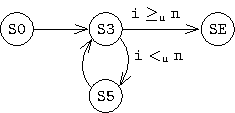
\includegraphics[scale=1.4]{chapters/figures/figMallocSpecCfg.pdf}}
\vspace{15pt}
\end{center}
\caption{\label{fig:llAllocSpecIRCFG}CFG of \SpecL{} program}
\end{subfigure}%
&
\begin{subfigure}[b]{0.5\textwidth}
\begin{center}
{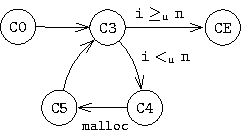
\includegraphics[scale=1.4]{chapters/figures/figMallocCCfg.pdf}}
\end{center}
\caption{\label{fig:llAllocCCFG}CFG of C program}
\end{subfigure}%
\\
\end{tabular}
\caption{\label{fig:mallocSpecCFGAndCCFG}CFG representation of Spec and C IRs shown in \cref{fig:llAllocSpecIR,fig:llAllocCIR} for the {\tt mk\_list} procedures in \cref{fig:llAllocSpec,fig:llAllocC} respectively.}
\end{figure}


Consequently, we are interested in proving that given $\sv{n} = \cv{n}$ at the procedure entries,
$\sv{ret} \indEq{} \lifted{list}{\mem{}}{lnode}{\cv{ret}}$ holds at the exits of both procedures.
Before going into the proof method,
we first introduce an alternate representation of IR, called the Control-Flow Graph (CFG for short).
\Cref{fig:llAllocSpecIRCFG,fig:llAllocCCFG} show the CFG representation of the \SpecL{} and C IRs
in \cref{fig:llAllocSpecIR,fig:llAllocCIR} respectively.
The CFG representation is fundamentally a labeled transition system representation of the corresponding IR,
and is further explored in \cref{sec:ir}.
In essence, each node represents a PC location of its IR, and each edge represents (possibly conditional)
transition between PCs through instruction execution.
For brevity, we often represent a sequence of instructions with a single edge, e.g.,
in \cref{fig:llAllocCCFG}, the edge \cpath{5,3} represents the path \cpath{5,6,7,8,3} in \cref{fig:llAllocCIR}.

\begin{figure}[H]
\begin{tabular}{cc}
\begin{subfigure}[b]{1\textwidth}
\begin{center}
{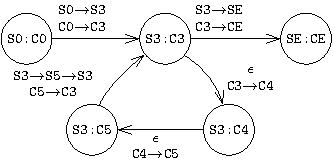
\includegraphics[scale=1.2]{chapters/figures/figMallocProductCfg.pdf}}
\end{center}
\end{subfigure}%
\end{tabular}
\caption{\label{fig:llAllocProductCFG}Product-CFG between \cref{fig:llAllocSpecIRCFG,fig:llAllocCCFG}}
\end{figure}


A common approach for showing equivalence between a pair of procedures involve finding a
bisimulation relation across the said procedure-pair.
Intuitively, a bisimulation relation (a) correlates program transitions across the specification
and implementation procedures, and (b) asserts inductively-provable invariants between
the machine states of the two procedures at the endpoints of each correlated transition \cite{pnueli98}.
Bisimulation itself can be represented as a program, called a {\em product program} \cite{covac}
and its CFG representation is called a {\em product}-CFG.
\Cref{fig:llAllocProductCFG} shows a product-CFG between the \SpecL{} and C {\tt mk\_list} procedures
in \cref{fig:llAllocSpecIRCFG,fig:llAllocCCFG} respectively.

\begin{table}[H]
\begin{center}
\caption{\label{tab:llproductInv}Node Invariants for Product-CFG in \cref{fig:llAllocProductCFG}}
\setlength{\belowcaptionskip}{-30pt}
\begin{footnotesize}
\begin{tabular}{|c|llll|}
\hline
\tt PC-Pair & \multicolumn{4}{c|} {\tt Invariants} \\
\hline
\hline
${\tt (S0:C0)}$ &
\multicolumn{4}{l|} {\Tstrut ${\tt { \circled{P}}\  n_{S}=n_{C}}$} \\
${\tt (S3:C3)}$ &
\Tstrut  ${\tt {\scriptsize \circled{I1}}\  n_{S}=n_{C}}$ & ${\tt {\scriptsize \circled{I2}}\  i_{S}=i_{C}}$ & ${\tt {\scriptsize \circled{I3}}\  i_{S} \leq_{u} n_{S}}$ & ${\tt {\scriptsize \circled{I4}}\  l_{S}\indEq{}Clist^{lnode}_{m}(l_{C})}$ \\
${\tt (S3:C4)\ (S3:C5)}$ &
\Tstrut  ${\tt {\scriptsize \circled{I5}}\  n_{S}=n_{C}}$ & ${\tt {\scriptsize \circled{I6}}\  i_{S}=i_{C}}$ & ${\tt {\scriptsize \circled{I7}}\  i_{S} <_{u} n_{S}}$ & ${\tt {\scriptsize \circled{I8}}\  l_{S}\indEq{}Clist^{lnode}_{m}(l_{C})}$ \\
${\tt (SE:CE)}$ &
\multicolumn{4}{l|} {\Tstrut  ${\tt {\circled{E}}\  ret_{S}\indEq{}Clist^{lnode}_{m}(ret_{C})}$} \\
\hline
\end{tabular}
\end{footnotesize}
\end{center}
\end{table}


At each node of the product-CFG, {\em invariants} relate the states of the \SpecL{} and C procedures respectively.
\Cref{tab:llproductInv} lists invariants for the product-CFG in \cref{fig:llAllocProductCFG}.
At the start node (\scpc{0}{0}) of the product-CFG, the precondition (labeled \circled{\small P})
ensures equality of input arguments \sv{n} and \cv{n} at the procedure entries.
Inductive invariants (labeled \circled{I}) need to be inferred at
each intermediate product-CFG node (e.g., (\scpc{3}{3})) relating both programs' states.
For example, at node (\scpc{3}{5}), \circled{\small I6} $\sv{i} = \cv{i}$ is an inductive invariant.
The inductive invariant \circled{\small I4} $\sv{l} \indEq{} \lifted{list}{\mem{}}{lnode}{\cv{l}}$
is another example of a \recursiveRelation{} and asserts equality between the intermediate \SpecL{} and C lists
at their respective loop heads.
Assuming that the precondition (\circled{\small P}) holds at the entry node (\scpc{0}{0}),
a bisimulation check involves checking that the inductive invariants hold too,
and consequently the postcondition (\circled{\small E}) holds at the exit node (\scpc{E}{E}).
Checking correctness of a bisimulation relation involves checking whether an invariant holds (along with many other things).
These checks result in proof queries which must be discharged by a solver (aka theorem prover).

\section{Our Contributions}
\label{sec:contribs}
As previously summarized in \cref{sec:motivatingexample}, an algorithm to find a bisimulation based proof of equivalence
between a \SpecL{} and C procedure involves three major algorithms:
\curved{A1} An algorithm for construction of a product-CFG by correlating program executions
across the \SpecL{} and C programs respectively.
\curved{A2} An algorithm for identification of inductively-provable invariants at intermediate correlated PCs.
\curved{A3} An algorithm for solving proof obligations generated by \curved{A1} and \curved{A2} algorithms.
Next we list our major contributions.

\begin{itemize}
\item Proof Discharge Algorithm: Solving proof obligations (\curved{A3}) involving \recursiveRelations{}
(generated by \curved{A1} and \curved{A2}) is quite interesting and forms our primary contribution.
We describe a {\em sound} proof discharge algorithm capable of tackling proof obligations involving
\recursiveRelations{} using off-the-shelf SMT solvers. Our proof discharge algorithm is also capable of
reconstruction of counterexamples for the original proof query from models returned by the individual SMT queries.
These counterexamples form the foundation of counterexample-guided heuristics for \curved{A1} and \curved{A2} algorithms
as we will see soon.
As part of our proof discharge algorithm,
we reformulate equality of ADT values (i.e. \recursiveRelations{}) as equivalence of programs
and discharge these proof queries using a nested (albeit much simpler) equivalence check.

\item Spec-to-C Automatic Equivalence Checker Tool: Our second contribution is \toolName{}, a {\em sound} equivalence checker tool
capable of proving equivalence between a \SpecL{} and a C program automatically.
\toolName{} either successfully finds a bisimulation relation implying equivalence or it provides a (sound but incomplete) unknown verdict.
\toolName{} is based on the Counter tool\cite{oopsla20} and uses specialized versions of (a) counterexample-guided correlation algorithm for
incremental construction of a product-CFG (\curved{A1}) and (b) counterexample-guided invariant inference algorithm
for inference of inductive invariants at correlated PCs in the (partially constructed) product-CFG (\curved{A2}).
\toolName{} discharges required verification conditions (i.e. proof obligations) using our Proof Discharge Algorithm.
The counterexamples generated by the proof discharge algorithm help steer the search algorithms \curved{A1} and \curved{A2}.
\end{itemize}

\section{Organization of the Thesis}
\label{sec:outline}
TODO

The rest of this thesis is divided into five chapter.
We begin with a thorough presentation of the topics discussed till now.
This includes our \SpecL{} language, the logical representation along with
bisimulation in the context of equivalence checking.
We finish with a discussion on the generated proof obligations and their language.

The next chapter illustrates our proof discharge algorithm using multiple \SpecL{} and C
sample programs.

Next, we give a detailed description of our automatic \SpecL{}-to-C equivalence checker tool \toolName{}
along with its most crucial components.

We finish with a comprehensive evaluation of \toolName{} and note its limitations.
We conclude our work by reiterating the key ideas presented alongside some related work.
\section{Conclusion}
\label{sec:conclusion}
As introduced in \cref{sec:syn-intro}, most of the current solutions
to the problem of equivalence checking between a functional specification
and a C program relies heavily on manually provided correlation, inductive
invariants as well as proof assistants for discharging said obligations.
While the size of programs considered in our work is quite small,
we hope the ideas in \toolName{} will help
automate the proofs for such systems to some degree.

Prior work on push-button verification of specific
systems \cite{fscq,hyperkernel,serval,verifiedBPF}
involves a combination of careful system design and
automatic verification tools like SMT solvers.
Constrained Horn Clause (CHC) Solvers \cite{CHCeq}
encode verification conditions of programs containing loops and recursion,
and raise the level of abstraction for automatic proofs.
Comparatively, \toolName{} further raises the level
of abstraction for automatic verification from
SMT queries and CHC queries to automatic discharge of
proof obligations involving \recursiveRelations{}.

A key idea in \toolName{} is the conversion of proof
obligations involving \recursiveRelations{} to
bisimulation checks. Thus, \toolName{} performs {\em nested}
bisimulation checks as part of a `higher-level'
bisimulation search. This approach of
identifying \recursiveRelations{} as invariants and using
bisimulation to discharge the associated
proof obligations may have applications
beyond equivalence checking.

\vspace{-12px}
\section{Outline of the Thesis}
\vspace{-10px}
\label{sec:outlinethesis}
\textbf{Chapter 1} of the thesis contains a general introduction to the research problem of verification C programs against a functional specification.
We take a C program and its analogue in a safe functional language, and contrast their differences. This helps us motivate the problem and its solution.
We finish with our contributions.

In \textbf{Chapter 2}, we constrain the programs being considered by formulating the problem statement. This helps us define the scope of our solution.
We introduce a custom minimal functional language called `Spec' and define the necessary terminology used in the rest of the thesis.

\textbf{Chapter 3} starts with background on program equivalence, bisimulation relation and product program.
The rest of the chapter gradually introduces our first contribution: A Proof Discharge Algorithm and related sub-procedures with the help
of two example programs. We also introduce a program representation of values, called `reconstruction program'.

Next, we formalize previously discussed topics in \textbf{Chapter 4}. We begin with the specification of our custom language `Spec'.
We give a detailed description of (a) a counterexample-guided search algorithm for finding a bisimulation relation and (b) a counterexample-guided
invariant inference procedure. There two procedures with our proof discharge algorithm allow automatic end-to-end equivalence checking.
We formalize handling of procedure calls in `Spec' as well as C, and finish with a dataflow analysis formulation of a pointer analysis
used by our equivalence checker.

\textbf{Chapter 5} introduces a program graph representation of values, called `deconstruction procedure', similar to `reconstruction procedure' as introduced in \textbf{Chapter 3}.
We motivate it by listing its advantages and give an algorithm to convert expressions to this representation.
This helps us simplify our proof discharge algorithm.

In \textbf{Chapter 6}, we introduce our automatic equivalence checker tool named \toolName{}, based on our proof discharge algorithm
and counterexample-guided search procedures.
\toolName{} is evaluated on a large variety of C programs involving lists, strings, trees and matrices.
This includes C programs taken from C library implementations as well as manually written programs. We show that our equivalence checker is able
to prove equivalence of a single specification with multiple of C implementations, each varying in its data layouts and algorithmic
strategies.

Finally, \textbf{Chapter 7} discusses the limitations of our algorithm and compares it with some related work. We note our major ideas and finish with
some potential future improvements to our algorithm.
\section*{Publications Based on Research Work}
\label{sec:publications}
% \begin{enumerate}
%     \item A. Bhardwaj, MVP. Srivastava, V. Wilson, A. Mehndiratta, V. Vishnu, and R. Garg, “Critical analysis of differentiation between ischemic stroke and hemorrhagic stroke in resource limited settings: A systematic review,” in \textit{International Journal of Stroke}, vol. 16, pp. 192–192, 2021.
    
%     \item A. Bhardwaj, Y. Antil, A. Chadha, MVP. Srivastava, V. Wilson, A. Mehndiratta, V. Vishnu, and R. Garg, “On evaluating the potential of machine learning for effective classification of ischemic stroke and hemorrhagic stroke in resource limited settings,” in \textit{International Journal of Stroke}, vol. 16, pp. 195–196, 2021.
    
%     \item A. Bhardwaj, M. P. Srivastava, P. W. Vinny, A. Mehndiratta, V. Y. Vishnu, and R. Garg, “Machine learning based reanalysis of clinical scores for distinguishing between ischemic and hemorrhagic stroke in low resource setting,” \textit{medRxiv}, 2022 Submitted: \textit{Journal of the Neurological Sciences}
    
%     \item Title: Clinical identification of stroke and stroke type via clinical attributes and gait analysis in resource-constrained environment. Under Review: \textit{World Stroke Congress 2022}
    
%     \item Title: STROKE-ASSIST: A Novel Machine Learning Framework For Stroke Type Identification In Resource Constrained Settings That Operates With Missing Data. (To be submitted to JAMA Neurology.)
    
%     \item Title: Sparsely Correlated Oblique Sparse Factor Model via Doubly-Penalized Matrix Decomposition. (To be submitted to NeurIPS or ICML.)
    
%     \item Title: STROKE-VISION: A Visual Data Collection Protocol for Enabling Automated Detection of Stroke (To be submitted to International Journal of Stroke.)

% \end{enumerate}
\begin{singlespace}
	\bibliographystyle{abbrvnat}
	\bibliography{refs}
\end{singlespace}
%  %%%%%%%%%%%%%%%%%%%%%%%%%%%%%%%%%%%%%%%%%%%%%%%%%%%%%%%%%%%%
% Appendices.

\appendix
% \section{Appendix A.1}

%%%%%%%%%%%%%%%%%%%%%%%%%%%%%%%%%%%%%%%%%%%%%%%%%%%%%%%%%%%%
% About the Author.

% \section*{About the Author}


\end{document}	